\chapter{Generalised Linear Models \& Gradient Descent}

\sn{Course Structure}{This part's additional materials will only be helpful after Chapter 6. Divorcing GLMs from their probabilistic context is rarely done, and is only done here for pedagogical purposes.}

Thus far we have utilised basis expansion to improve linear models. These models, especially with polynomial basis expansion, are great for modelling variables $y$ that vary constantly with respect to either their features or basis-expanded features.  Even though they are a arbitrarily powerful function approximator (formal statement will be discussed later in the course), they run the risk of overfitting (Chapter 5).  We motivate that data assumptions and model assumptions are different.

\defb{Gradient Notation}{
    In this course, vectors are assumed to be column vectors by default:

    \[
        \bm{b} \in \mathbb{R}^n = \bm{b} \in \mathbb{R}^{n \times 1}
    \]

    Gradients of vector-valued functions are, by convention, row vectors:

    \[
        f(\bm{b}) : \mathbb{R}^n \to \mathbb{R} \implies \nabla_{\bm{b}} f(\bm{b}) \in \mathbb{R}^{1 \times n}
    \]

    \[
        f(\bm{b}) : \mathbb{R}^n \to \mathbb{R}^m \implies \nabla_{\bm{b}} f(\bm{b}) \in \mathbb{R}^{m \times n}
    \]

    This layout is referred to as the "numerator" layout.
}

\section{Generalised Linear Models}
Generalised Linear Models use a single non-linear funciton to encode our beliefs about the output of our model, with the general form:

\begin{equation}
    \bm{y} = g^{-1}(\theta ^\top \bm{x})
\end{equation}

$g$ is the ``link'' function, traditionally associated with a probability density function from the exponential family.  However, we will later discuss when this interpretation will become very useful. A brief overview why GLMs are useful:
\begin{itemize}
    \item They are flexible with different data distributions. Standard linear regression assumes a normal distribution of errors or outputs, but GLMs can model other distributions such as Poisson, Bernoulli/Binomial, or Poisson.
    \item Linear regression assumes that the output $y$ is directly a linear function of the inputs (which we can transform from $x$ as part of the basis expansion). GLM assumes that some transformation of $y$ via the link function $g$ is linear in the inputs. It transforms the output variable instead of the input variables.
\end{itemize}


\subsection{Poisson Regression}
In many applications, we want to predict count information: e.g. how many people in a house, or the number of accidents in a city yearly. However linear regression models do not have restricted outputs and can predict negative values. Poisson Regression is a GLM that addresses this. \bigskip

Example: I want to predict the number of times a ship will get damaged in a particular period, given some information about the ship.

\begin{table}[h!]
    \centering
    \begin{tabular*}{\linewidth}{@{\extracolsep{\fill}} l l l r r}
        \toprule
        \textbf{TYPE} & \textbf{YEAR} & \textbf{PERIOD} & \textbf{MONTHS} & \textbf{Y} \\
        \midrule
        b & 1965-69 & 1975-79 & 20370 & 53 \\
        b & 1970-74 & 1960-74 & 7064  & 12 \\
        b & 1970-74 & 1975-79 & 13099 & 44 \\
        b & 1975-79 & 1960-74 & 0     & 0  \\
        b & 1975-79 & 1975-79 & 7117  & 18 \\
        b & 1960-64 & 1960-74 & 44882 & 39 \\
        b & 1960-64 & 1975-79 & 17176 & 29 \\
        b & 1965-69 & 1960-74 & 28609 & 58 \\
        c & 1960-64 & 1960-74 & 1179  & 1  \\
        c & 1960-64 & 1975-79 & 552   & 1  \\
        \bottomrule
    \end{tabular*}
    \caption{Types of damages and the number of times they occurred in a particular period.}
    \label{tab:example_table}
\end{table}

Consider a design matrix $\bm{X}' \in \mathbb{R}^{n \times m}$ and response variables are collected into response vector $\bm{y} \in \mathbb{R}^n$. \bigskip

We augment the design matrix, adding a 1 to the end of each vector (affine basis expansion).

\begin{equation}
    \bm{X}' \rightarrow \bm{X} \in \mathbb{R}^{(n+1) \times m}
\end{equation}

To achieve the desired strictly positive co-domain, we simply exponentiate:

\begin{equation}
    \hat{\bm{y}} = \exp(\bm{X} {\theta})
\end{equation}

The loss function is given by:

\begin{equation}
    \mathcal{L}(\theta) = \sum_{i=1}^{m} \left( y^{(i)} \bm{x}^{(i)^\top} \theta - \exp(\bm{x}^{(i)^\top} \theta) \right) - \sum_{i=1}^{m} \log\left(y^{(i)}!\right)
\end{equation}

The full context and derivation of this loss function will be covered in later chapters (early hint: it is the log-likelihood). This loss function does not have a closed-form solution. \bigskip

Instead, we can try to use MSE loss instead to find its gradient:

\begin{align*}
    \mathcal{L}(\theta) & = \frac{1}{m} (\hat{y} - y)^2                            \\
                        & = \frac{1}{m} (\exp(\bm{X}\theta) - y)^2                 \\
                        & \propto (\exp(\bm{X}\theta) - y)^2                       \\
                        & = (\exp(\bm{X}\theta) - y)^\top (\exp(\bm{X}\theta) - y)
\end{align*}

To compute the gradient, the loss is expressed as a summation:

\[
    \mathcal{L}(\theta) = \sum_{i=1}^{k} (\exp(\bm{X}_{i,:}^\top \theta) - y_i)^2
\]

where \(\bm{X}_{i,:}^\top\) is the \(i\)-th row of \(\bm{X}\). Applying the chain rule:

\[
    \frac{\partial}{\partial \theta} \left( \exp(\bm{X}_{i,:}^\top \theta) - y_i \right)^2 = 2 (\exp(\bm{X}_{i,:}^\top \theta) - y_i) \cdot \frac{\partial}{\partial \theta} \exp(\bm{X}_{i,:}^\top \theta)
\]

The derivative of \(\exp(\bm{X}_{i,:}^\top \theta)\) with respect to \(\theta\) is:

\[
    \frac{\partial}{\partial \theta} \exp(\bm{X}_{i,:}^\top \theta) = \exp(\bm{X}_{i,:}^\top \theta) \cdot \bm{X}_{i,:}^\top
\]

Thus, the gradient of each term is:

\[
    \frac{\partial}{\partial \theta} \left( \exp(\bm{X}_{i,:}^\top \theta) - y_i \right)^2 = 2 (\exp(\bm{X}_{i,:}^\top \theta) - y_i) \cdot \exp(\bm{X}_{i,:}^\top \theta) \cdot \bm{X}_{i,:}^\top
\]

Summing over all data points:

\[
    \nabla_\theta \mathcal{L}(\theta) = 2 \sum_{i=1}^{k} (\exp(\bm{X}_{i,:}^\top \theta) - y_i) \cdot \exp(\bm{X}_{i,:}^\top \theta) \cdot \bm{X}_{i,:}^\top
\]

In matrix form:

\[
    \nabla_\theta \mathcal{L}(\theta) = 2 \left( (\exp(\bm{X}\theta) - \bm{y}) \odot \exp(\bm{X}\theta) \right)^\top \bm{X}
\]

Here, \(\odot\) denotes element-wise multiplication.

\subsection{Logistic Regression}
In many applications, we would like to predict the class of a particular input e.g. classifying if an email is spam or not. The simplest case is binary classification, where the output is either 0 or 1. We take $\bm{y} \in [0,1]$ in this case.

\begin{figure}[h!]
    \centering
    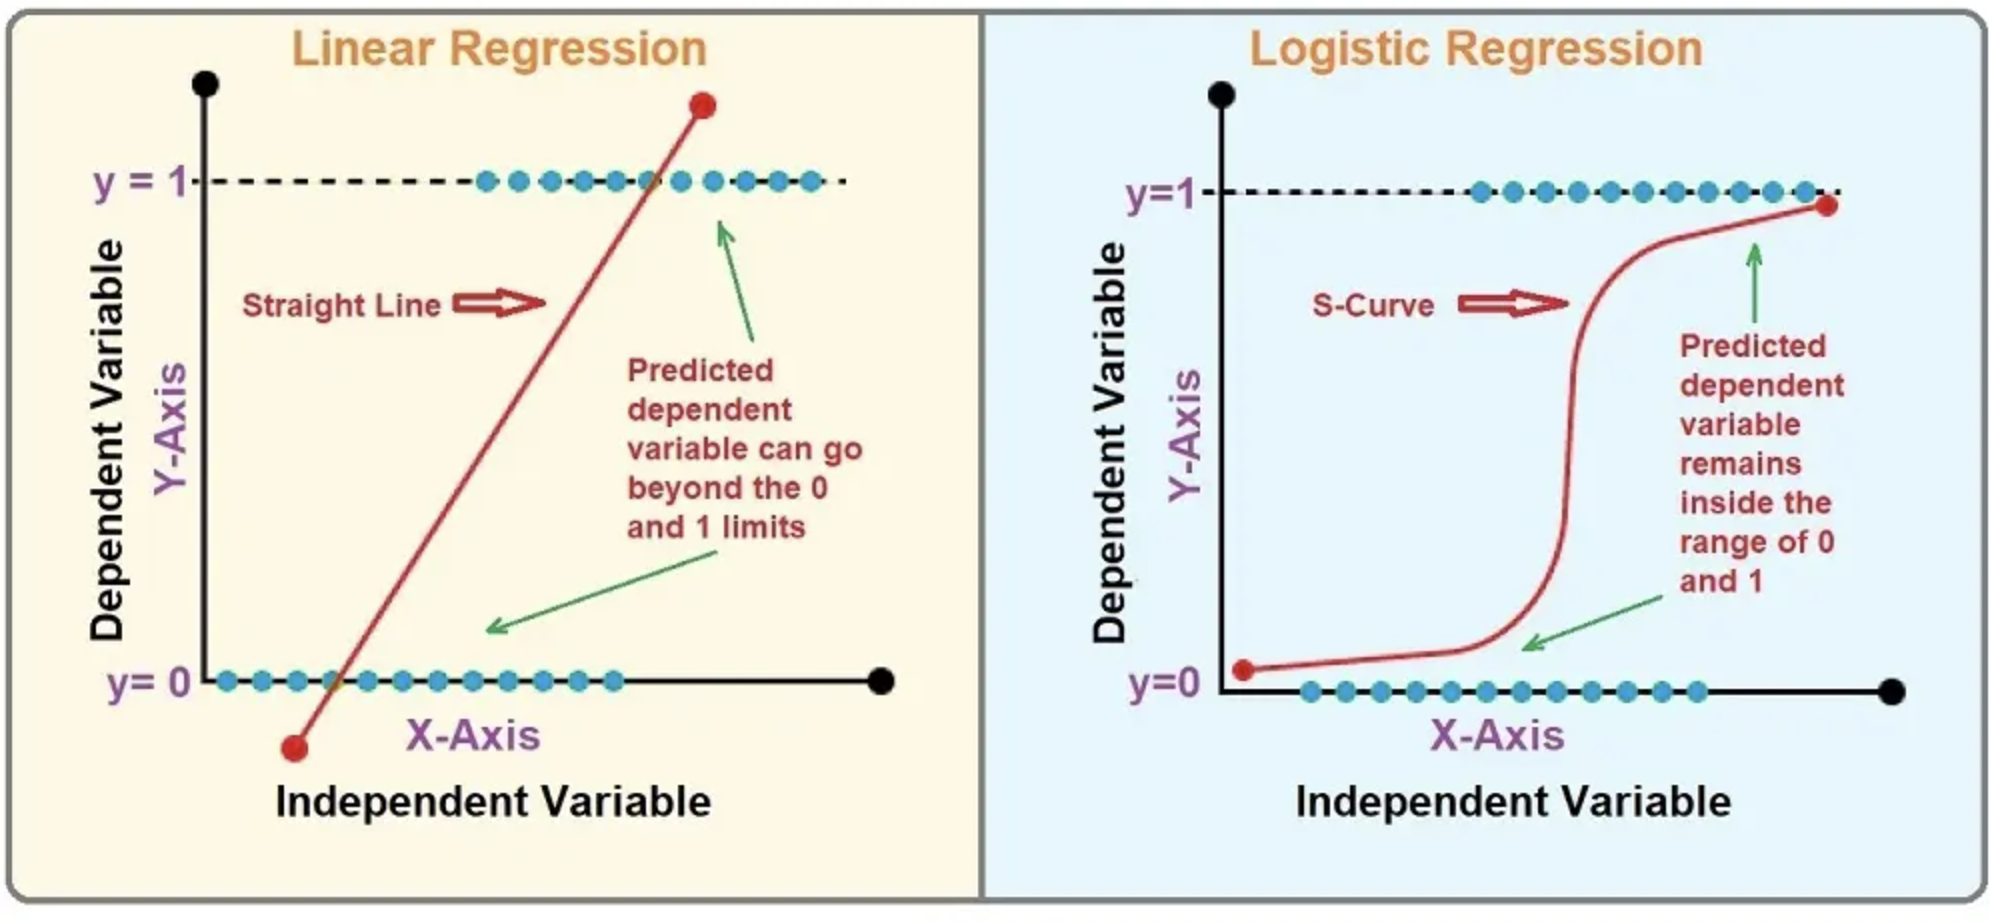
\includegraphics[width=1\textwidth]{img/3_lr_vs_logistic.png}
    \caption{Using a contrived, unbalanced dataset, we visualise an intuitive case where the non-linearity in  logistic regression helps us model the data more accurately compared to linear regression.}
\end{figure}


Consider a design matrix $\bm{X}' \in \mathbb{R}^{n \times m}$ and response variables are collected into response vector $\bm{y} \in \mathbb{R}^n$ where entries $y_i \in \{0,1\}$. \bigskip

We augment the design matrix as usual, adding a 1 to the end of each vector (affine basis expansion).

\begin{equation}
    \bm{X}' \rightarrow \bm{X} \in \mathbb{R}^{(n+1) \times m}
\end{equation}

We then apply the logistic function so that the range of the output is $[0,1]$:
\begin{equation}
    \sigma(x) = \frac{1}{1 + \exp(-x)}
\end{equation}

The loss function we desire is the negative log-likelihood for the Bernoulli distribution which is:

\[
    \mathcal{L}(\theta) = -\frac{1}{m} \sum_{i=1}^{m} \left( y^{(i)} \log(\sigma(\theta^\top \bm{x}^{(i)})) + (1 - y^{(i)}) \log(1 - \sigma(\theta^\top \bm{x}^{(i)})) \right)
\]

where \(\sigma(x) = \frac{1}{1 + \exp(-x)}\) is the logistic function. \bigskip

Since the minimiser of this equation cannot be solved in closed form, we use numerical methods such as gradient descent.

The gradient of the loss function with respect to \(\theta\) is:

\[
    \nabla_\theta \mathcal{L}(\theta) = -\frac{1}{m} \sum_{i=1}^{m} \left( y^{(i)} (1 - \sigma(\theta^\top \bm{x}^{(i)})) - (1 - y^{(i)}) \sigma(\theta^\top \bm{x}^{(i)}) \right) \bm{x}^{(i)}
\]

This simplifies to:

\[
    \nabla_\theta \mathcal{L}(\theta) = -\frac{1}{m} \sum_{i=m}^{k} \left( y^{(i)} - \sigma(\theta^\top \bm{x}^{(i)}) \right) \bm{x}^{(i)}
\]


\refb{Linear Models for Classification}{
\textbf{Linear models for classification, Chapter 4.1 - 4.1.3 (page 179) Bishop (2006).}
\bigskip

Note that we did not use the MSE approach here– for a more detailed discussion on why this is not ideal, refer to the above reference. \smallskip


\begin{center}
    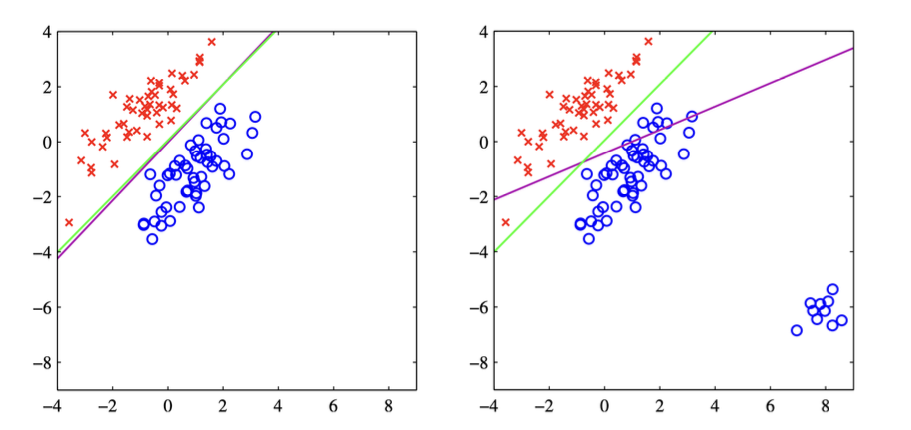
\includegraphics[width=1\textwidth]{img/3_logistic_outliers.png}
\end{center}
{\small Figure and caption text from Bishop 2006: The left plot shows data from two classes, denoted by red crosses and blue circles, together with the decision boundary found by least squares (magenta curve) and also by the logistic regression model (green curve). The right-hand plot shows the corresponding results obtained when extra data points are added at the bottom left of the diagram, showing that least squares is highly sensitive to outliers, unlike logistic regression.}

\bigskip





Why we do not use the MSE loss:
\begin{itemize}
    \item The MSE itself is meant for continuous output values, so it does not make sense to use it for binary classification.
    \item The squaring of error in MSE amplifies the impact of large errors or outliers, thus a few outliers can disproportionately influence the whole model.
\end{itemize}


}

\section{Gradient Descent}

Gradient descent is the core algorithm behind the \textit{learning} portion of many ML algorithms, by fining the minimum of a (loss) function The idea is to iteratively take steps in the direction of the steepest descent, which is determined by the gradient of the function. The gradient is denoted by \(\nabla\), with a subscript indicating the variable we are differentiating with respect to.

The basic form of gradient descent is:

\[
    \theta^{(t+1)} = \theta^{(t)} + \alpha \nabla_\theta \mathcal{L}(f^\theta, \bm{X}, \bm{y}),
\]

where \(\alpha\) is the learning rate, and \(\theta^{(0)} \sim \mathcal{N}(0, 1)\).\bigskip


We interpret (in the two-dimensional weight case) \(\mathcal{L}(f^\theta, \bm{X}, \bm{y})\) as a height we want to minimise, and visualise \(\theta\) as a puck being pushed in the direction that lowers the height.\bigskip

Some factors that affect the convergence of gradient descent are:
\begin{itemize}
    \item Learning rate: If the learning rate is too high, the puck may overshoot the minimum. If it is too low, the puck may take too long to reach the minimum.
    \item Iterations: A sufficient number of iterations is needed to reach the minimum – if not enough, the optimal loss is not achieved.
\end{itemize}


\begin{figure}[h!]
    \centering
    % First subfigure
    \begin{subfigure}[b]{0.49\linewidth}
        \centering
        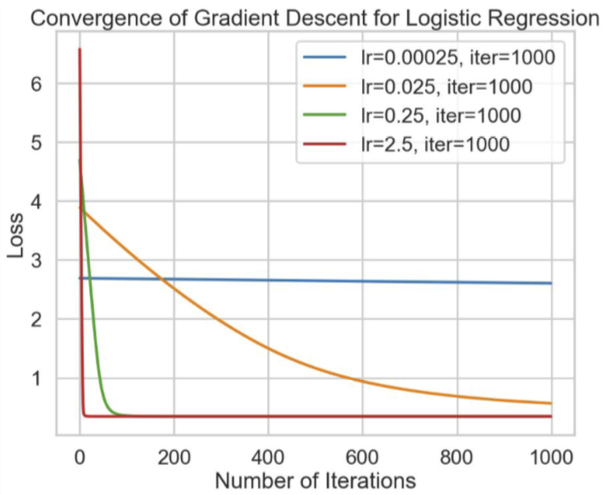
\includegraphics[width=\linewidth]{img/3_logr_gd.png}
        \caption{Convergence of the loss during gradient descent for logistic regression.}
        \label{fig:logr_gd}
    \end{subfigure}
    % Second subfigure
    \begin{subfigure}[b]{0.49\linewidth}
        \centering
        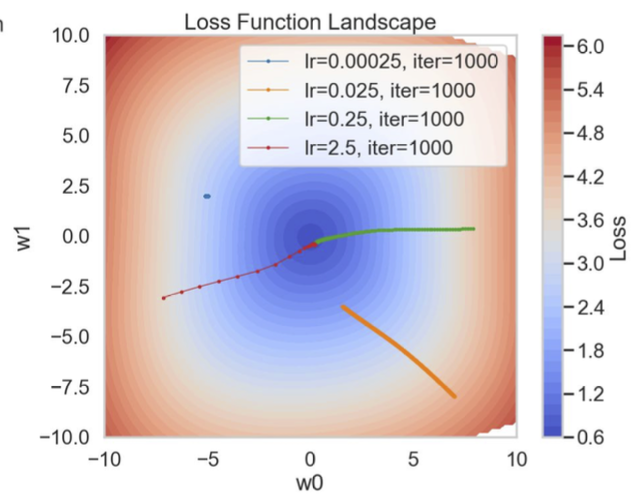
\includegraphics[width=\linewidth]{img/3_logr_loss_function_landscape.png}
        \caption{Loss function landscape and path of the parameter as it moves.}
        \label{fig:logr_loss_landscape}
    \end{subfigure}

    \caption{Effect of learning rate on logistic regression training. (a) The convergence of the loss over iterations, interpreted as the height of the puck in the bowl. (b) A visualisation of the parameter's path in the loss function landscape.}
    \label{fig:logr_learning_rate_effect}
\end{figure}

\begin{figure}[h!]
    \centering
    % First subfigure
    \begin{subfigure}[b]{0.49\linewidth}
        \centering
        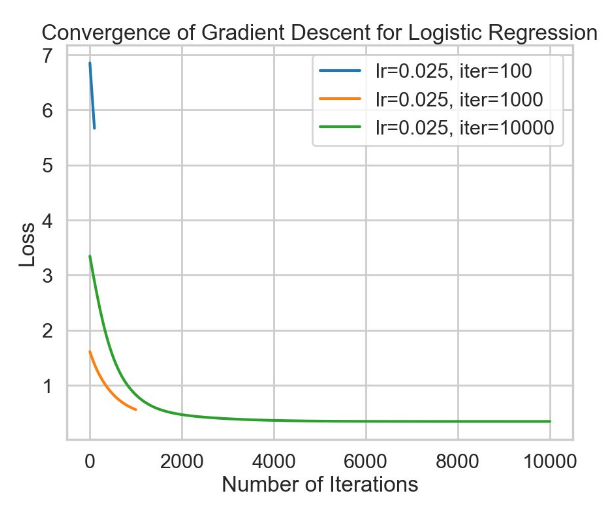
\includegraphics[width=\linewidth]{img/3_logr_gd_iters.png}
        \caption{Convergence of the loss during gradient descent for logistic regression with different numbers of iterations.}
        \label{fig:logr_gd_iters}
    \end{subfigure}
    % Second subfigure
    \begin{subfigure}[b]{0.49\linewidth}
        \centering
        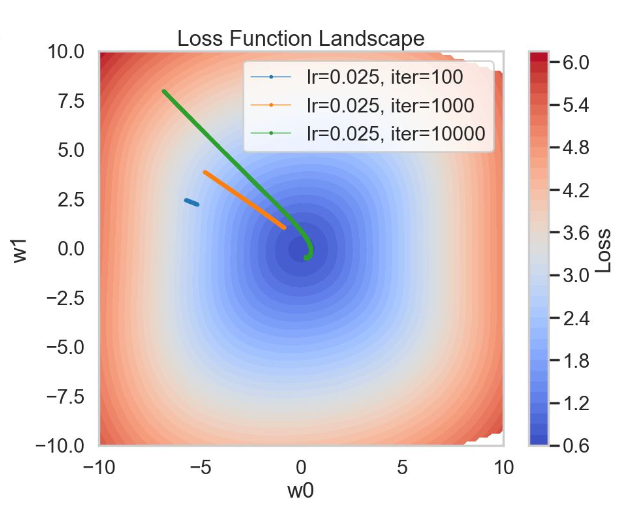
\includegraphics[width=\linewidth]{img/3_logr_loss_function_landscape_iters.png}
        \caption{Loss function landscape and parameter's path with different iterations.}
        \label{fig:logr_loss_landscape_iters}
    \end{subfigure}

    \caption{Effect of number of iterations on the learning of our logistic regression model. (a) The convergence of the loss over iterations, interpreted as the height of the puck in the bowl. (b) A visualization of the parameter's path in the loss function landscape for different iterations.}
    \label{fig:logr_iterations_effect}
\end{figure}

\newpage
\subsection{Complexity of OLS Closed-Form Solution}
It is awkward to compare Ordinary Least Squares (OLS) to Gradient Descent (GD) in Generalised Linear Models (GLM), as we cannot directly use the OLS in GLMs. \footnote{OLS assumes the errors in the model are normally distributed and have constant variance (called homoscedasticity), a common regression assumption. But Generalised Linear Models don't have this condition, and errors can be distributed via the Poisson, binomial, or exponential families. GLMs use Maximum Likelihood Estimation (MLE) instead of the OLS, which will be explained in later chapters. } \bigskip

We can, however, consider the complexity of Ordinary Least Squares (OLS) with Gradient Descent (GD) for Generalised Linear Models (GLMs). \bigskip


First, consider the OLS closed-form solution:
\[
    \theta = (\bm{X}^\top \bm{X})^{-1} \bm{X}^\top \bm{y}
\]

\begin{enumerate}
    \item The matrix product $\bm{X}^\top \bm{X}$ involves multiplying two matrices \( A \in \mathbb{R}^{n \times m} \) and \( B \in \mathbb{R}^{m \times n} \), which has the general form:
          \[
              \bm{C}_{i,j} = \sum_{k=1}^{l} \bm{A}_{i,k} \bm{B}_{k,j}
          \]
          \begin{itemize}
              \item Since $k$ is our dummy index, it gets summed over $l$ times.
              \item It is repeated for each element in the resulting matrix $\bm{C}$.
              \item Remember, the data matrix $\bm{X}$ is of size \( n \times m \), so that's \( n \) features and \( m \) samples.
          \end{itemize}
          This operation has a complexity of \( O(n l m) \).

          \begin{figure}
              \centering
              \begin{tikzpicture}[scale=0.5]

                  % Matrix A
                  \matrix[matrix of math nodes,left delimiter={[},right delimiter={]}, nodes={font=\small}, inner sep=0.5pt, row sep = 15pt, column sep = 0pt] (A) {
                          A_{1,1} & A_{1,2} & \dots & A_{1,m} \\
                          A_{2,1} & A_{2,2} & \dots & A_{2,m} \\
                          \vdots  & \vdots  & \ddots & \vdots \\
                          A_{n,1} & A_{n,2} & \dots & A_{n,m} \\
                      };

                  % Matrix B
                  \matrix[matrix of math nodes,left delimiter={[},right delimiter={]}, nodes={font=\small}, inner sep=0.5pt, column sep = 5pt] (B) [right=1.5cm of A] {
                          B_{1,1} & B_{1,2} & \dots & B_{1,n} \\
                          B_{2,1} & B_{2,2} & \dots & B_{2,n} \\
                          \vdots  & \vdots  & \ddots & \vdots \\
                          B_{m,1} & B_{m,2} & \dots & B_{m,n} \\
                      };

                  % Matrix C
                  \matrix[matrix of math nodes,left delimiter={[},right delimiter={]}, nodes={font=\small}, inner sep=0.5pt, row sep =15pt, column sep = 0pt] (C) [right=1.5cm of B] {
                          C_{1,1} & C_{1,2} & \dots & C_{1,n} \\
                          C_{2,1} & C_{2,2} & \dots & C_{2,n} \\
                          \vdots  & \vdots  & \ddots & \vdots \\
                          C_{n,1} & C_{n,2} & \dots & C_{n,n} \\
                      };

                  % Place the multiplication and equals signs with better spacing
                  \node at ($(A.east)+(1.7,0)$) {\large $\times$};
                  \node at ($(B.east)+(1.7,0)$) {\large $=$};

                  % Highlight the first row of A with light transparent red fill
                  \draw[thick, red, fill=red!30, fill opacity=0.3, rounded corners]
                  ($(A-1-1.north west)+(-0.1,0.1)$) -- ($(A-1-4.north east)+(0.1,0.1)$) --
                  ($(A-1-4.south east)+(0.1,-0.1)$) -- ($(A-1-1.south west)+(-0.1,-0.1)$) -- cycle;

                  % Highlight the first column of B with light transparent blue fill
                  \draw[thick, blue, fill=blue!30, fill opacity=0.3, rounded corners]
                  ($(B-1-1.north west)+(-0.1,0.1)$) -- ($(B-4-1.south west)+(-0.1,-0.1)$) --
                  ($(B-4-1.south east)+(0.1,-0.1)$) -- ($(B-1-1.north east)+(0.1,0.1)$) -- cycle;

                  % Highlight the top-left element of C with light transparent green fill
                  \draw[thick, green, fill=green!30, fill opacity=0.3, rounded corners]
                  ($(C-1-1.north west)+(-0.1,0.1)$) -- ($(C-1-1.north east)+(0.1,0.1)$) --
                  ($(C-1-1.south east)+(0.1,-0.1)$) -- ($(C-1-1.south west)+(-0.1,-0.1)$) -- cycle;

              \end{tikzpicture}
              \caption{Matrix product \(\bm{X}^\top \bm{X}\) involves multiplying two matrices \(A \in \mathbb{R}^{n \times m}\) and \(B \in \mathbb{R}^{m \times n}\), resulting in a matrix \(C \in \mathbb{R}^{n \times n}\) with a complexity of \(O(n^2 m)\).}
          \end{figure}

          % \footnote{$\bm{X}^\top\bm{X}$ is really just a square matrix, we only keep $n$ and $m$ separate to understand which side of the index is being used.}

          Since \( \bm{X}^\top \bm{X} \) is of size \( n \times n \)  , the total complexity of computing this matrix product is \( O(n^2 m) \).

          \[
              \theta = \underbrace{(\bm{X}^\top \bm{X})^{-1}}_{n \times n}
              \underbrace{\bm{X}^\top}_{n \times m}
              \underbrace{\bm{y}}_{m \times 1}
          \]

    \item Next, matrix inversion for \( (\bm{X}^\top \bm{X})^{-1} \) (which is square) has complexity\footnote{There are several algorithms for matrix inversion that are better than cubic, but we stick to $O(n^3)$.}  \( O(n^3) \). Combining these operations, the current total complexity becomes:
          \[
              O(n^2 m + n^3)
          \]
    \item We multiply the \( \bm{X}^\top \bm{y} \) term. This is a matrix vector product between $\bm{A} \in \mathbb{R}^{n \times m}$ and $\bm{b} \in \mathbb{R}^{m \times 1}$ with complexity $O(mn)$ (see Figure \ref{fig:matrix_vector_product_1}).
          \[
              \bm{c}_j = \sum^n_{i=1} \bm{A}_{i,j} \bm{b}_i
          \]
          \begin{figure}[h!]
              \centering
              \begin{tikzpicture}[scale=0.5]

                  % Matrix X^T
                  \matrix[matrix of math nodes,left delimiter={[},right delimiter={]}, nodes={font=\small}, inner sep=0.5pt, column sep = 5pt] (X) {
                          X_{1,1} & X_{1,2} & \dots & X_{1,n} \\
                          X_{2,1} & X_{2,2} & \dots & X_{2,n} \\
                          \vdots  & \vdots  & \ddots & \vdots \\
                          X_{m,1} & X_{m,2} & \dots & X_{m,n} \\
                      };

                  % Vector y
                  \matrix[matrix of math nodes,left delimiter={[},right delimiter={]}, nodes={font=\small}, inner sep=0.5pt, row sep = 15pt, column sep = 0pt] (y) [right=1.5cm of X] {
                          y_{1} \\
                          y_{2} \\
                          \vdots  \\
                          y_{n} \\
                      };

                  % Result vector c
                  \matrix[matrix of math nodes,left delimiter={[},right delimiter={]}, nodes={font=\small}, inner sep=0.5pt] (c) [right=1.5cm of y] {
                          c_1 \\
                          c_2 \\
                          \vdots  \\
                          c_m \\
                      };

                  % Place the multiplication and equals signs with better spacing
                  \node at ($(X.east)!0.5!(y.west)$) {\large $\times$};
                  \node at ($(y.east)!0.5!(c.west)$) {\large $=$};

                  % Highlight the first row of X^T with light transparent red fill
                  \draw[thick, red, fill=red!30, fill opacity=0.3, rounded corners]
                  ($(X-1-1.north west)+(-0.1,0.1)$) -- ($(X-1-4.north east)+(0.1,0.1)$) --
                  ($(X-1-4.south east)+(0.1,-0.1)$) -- ($(X-1-1.south west)+(-0.1,-0.1)$) -- cycle;

                  % Highlight the first column of y with light transparent blue fill
                  \draw[thick, blue, fill=blue!30, fill opacity=0.3, rounded corners]
                  ($(y-1-1.north west)+(-0.1,0.1)$) -- ($(y-4-1.south west)+(-0.1,-0.1)$) --
                  ($(y-4-1.south east)+(0.1,-0.1)$) -- ($(y-1-1.north east)+(0.1,0.1)$) -- cycle;

                  % Highlight the top-left element of c with light transparent green fill
                  \draw[thick, green, fill=green!30, fill opacity=0.3, rounded corners]
                  ($(c-1-1.north west)+(-0.1,0.1)$) -- ($(c-1-1.north east)+(0.1,0.1)$) --
                  ($(c-1-1.south east)+(0.1,-0.1)$) -- ($(c-1-1.south west)+(-0.1,-0.1)$) -- cycle;

              \end{tikzpicture}
              \caption{Matrix-vector product for $\bm{X}^\top \bm{y}$}
              \label{fig:matrix_vector_product_1}
          \end{figure}

    \item We then multiply $(\bm{X}^\top \bm{X})^{-1}$ with \( \bm{X}^\top \bm{y} \). This is a matrix vector product between $\bm{A} \in \mathbb{R}^{n \times n}$ and $\bm{b} \in \mathbb{R}^{n \times 1}$ with complexity $O(n^2)$ (see Figure \ref{fig:matrix_vector_product_2}).
          \[
              \bm{c}_j = \sum^n_{i=1} \bm{A}_{i,j} \bm{b}_i
          \]
          \begin{figure}[h!]
              \centering
              \begin{tikzpicture}[scale=0.5]

                  % Matrix X^T
                  \matrix[matrix of math nodes,left delimiter={[},right delimiter={]}, nodes={font=\small}, inner sep=0.5pt, column sep = 5pt] (X) {
                          X_{1,1} & X_{1,2} & \dots & X_{1,n} \\
                          X_{2,1} & X_{2,2} & \dots & X_{2,n} \\
                          \vdots  & \vdots  & \ddots & \vdots \\
                          X_{n,1} & X_{n,2} & \dots & X_{n,n} \\
                      };

                  % Vector y
                  \matrix[matrix of math nodes,left delimiter={[},right delimiter={]}, nodes={font=\small}, inner sep=1pt, row sep = 15pt, column sep = 0pt] (y) [right=1.5cm of X] {
                          y_{1} \\
                          y_{2} \\
                          \vdots  \\
                          y_{n} \\
                      };

                  % Result vector c
                  \matrix[matrix of math nodes,left delimiter={[},right delimiter={]}, nodes={font=\small}, inner sep=1pt] (c) [right=1.5cm of y] {
                          c_1 \\
                          c_2 \\
                          \vdots  \\
                          c_n \\
                      };

                  % Place the multiplication and equals signs with better spacing
                  \node at ($(X.east)!0.5!(y.west)$) {\large $\times$};
                  \node at ($(y.east)!0.5!(c.west)$) {\large $=$};

                  % Highlight the first row of X^T with light transparent red fill
                  \draw[thick, red, fill=red!30, fill opacity=0.3, rounded corners]
                  ($(X-1-1.north west)+(-0.1,0.1)$) -- ($(X-1-4.north east)+(0.1,0.1)$) --
                  ($(X-1-4.south east)+(0.1,-0.1)$) -- ($(X-1-1.south west)+(-0.1,-0.1)$) -- cycle;

                  % Highlight the first column of y with light transparent blue fill
                  \draw[thick, blue, fill=blue!30, fill opacity=0.3, rounded corners]
                  ($(y-1-1.north west)+(-0.1,0.1)$) -- ($(y-4-1.south west)+(-0.1,-0.1)$) --
                  ($(y-4-1.south east)+(0.1,-0.1)$) -- ($(y-1-1.north east)+(0.1,0.1)$) -- cycle;

                  % Highlight the top-left element of c with light transparent green fill
                  \draw[thick, green, fill=green!30, fill opacity=0.3, rounded corners]
                  ($(c-1-1.north west)+(-0.1,0.1)$) -- ($(c-1-1.north east)+(0.1,0.1)$) --
                  ($(c-1-1.south east)+(0.1,-0.1)$) -- ($(c-1-1.south west)+(-0.1,-0.1)$) -- cycle;

              \end{tikzpicture}
              \caption{Matrix-vector product for $(\bm{X}^\top \bm{X})^{-1} \cdot (\bm{X}^\top \bm{y})$}
              \label{fig:matrix_vector_product_2}
          \end{figure}



          We have
          \begin{equation}
              \theta =
              \underbrace{
                  \underbrace{
                      \left( \underbrace{\bm{X}^\top \bm{X}}_{O(n^2m)} \right)^{-1}
                  }_{O(n^3)}
                  \underbrace{
                      \bm{X}^\top \bm{y}
                  }_{O(nm)}}_{O(n^2)}
          \end{equation}

          and our final complexity is \( O(n^2 m + n^3) \).\marginnote{This is because we had $O(nm + n^2m + n^2 + n^3) = O(n(m + nm + n) + n^3) \Rightarrow  O(n^2 m + n^3)$} This can be quite inefficient for large datasets where $m$ is large! We alleviate this by using stochastic gradient descent.

          \subsection{Complexity of Stochastic Gradient Descent}

          Instead of having to compute the full OLS solution by inverting the matrix, we can iterate towards an approximate solution by taking the gradient of the loss function and applying it to gradient descent. \bigskip

          We then can optimize the computation by sub-sampling a \textit{batch} of the data, leading to \textit{stochastic gradient descent (SGD)}. The gradient for linear regression is given by:
          \[
              \bm{X}^\top (\bm{X} \theta - \bm{y})
          \]

          The operations comprise:
          \begin{itemize}
              \item Matrix-vector multiplication \( \bm{X} \theta \) has a complexity of \( O(b n) \) if \( \bm{X} \in \mathbb{R}^{b \times n} \), where \( b \) is the batch size, $\theta \in \mathbb{R}^{n \times 1}$, $n$ is the number of features.

                    \[
                        \bm{c}_j = \sum_{i=1}^{n} \bm{X}_{i,j} \theta_i
                    \]

                    \begin{figure}

                        \centering
                        \begin{tikzpicture}[scale=0.5]

                            % Matrix X^T
                            \matrix[matrix of math nodes,left delimiter={[},right delimiter={]}, nodes={font=\small}, inner sep=1pt] (X) {
                                    X_{1,1} & X_{1,2} & \dots & X_{1,n}  \\
                                    X_{2,1} & X_{2,2} & \dots & X_{2,n}  \\
                                    \vdots  & \vdots  & \ddots & \vdots  \\
                                    X_{b,1} & X_{b,2} & \dots & X_{b,n}  \\
                                };

                            % Vector theta
                            \matrix[matrix of math nodes,left delimiter={[},right delimiter={]}, nodes={font=\small}, inner sep=1pt] (theta) [right=1.5cm of X] {
                                    \theta_{1} \\
                                    \theta_{2} \\
                                    \vdots  \\
                                    \theta_{n} \\
                                };

                            % Result vector c
                            \matrix[matrix of math nodes,left delimiter={[},right delimiter={]}, nodes={font=\small}, inner sep=1pt] (c) [right=1.5cm of theta] {
                                    c_1 \\
                                    c_2 \\
                                    \vdots  \\
                                    c_b \\
                                };

                            % Place the multiplication and equals signs with better spacing
                            \node at ($(X.east)!0.5!(theta.west)$) {\large $\times$};
                            \node at ($(theta.east)!0.5!(c.west)$) {\large $=$};

                            % Highlight the first row of X^T with light transparent red fill
                            \draw[thick, red, fill=red!30, fill opacity=0.3, rounded corners]
                            ($(X-1-1.north west)+(-0.1,0.1)$) -- ($(X-1-4.north east)+(0.1,0.1)$) --
                            ($(X-1-4.south east)+(0.1,-0.1)$) -- ($(X-1-1.south west)+(-0.1,-0.1)$) -- cycle;

                            % Highlight the first column of theta with light transparent blue fill
                            \draw[thick, blue, fill=blue!30, fill opacity=0.3, rounded corners]
                            ($(theta-1-1.north west)+(-0.1,0.1)$) -- ($(theta-4-1.south west)+(-0.1,-0.1)$) --
                            ($(theta-4-1.south east)+(0.1,-0.1)$) -- ($(theta-1-1.north east)+(0.1,0.1)$) -- cycle;

                            % Highlight the top-left element of c with light transparent green fill
                            \draw[thick, green, fill=green!30, fill opacity=0.3, rounded corners]
                            ($(c-1-1.north west)+(-0.1,0.1)$) -- ($(c-1-1.north east)+(0.1,0.1)$) --
                            ($(c-1-1.south east)+(0.1,-0.1)$) -- ($(c-1-1.south west)+(-0.1,-0.1)$) -- cycle;

                        \end{tikzpicture}
                    \end{figure}
              \item $(\bm{X} \theta - \bm{y}) \in \mathbb{R}^{b \times 1}$ is a vector subtraction, which has a complexity of \( O(b) \).
              \item Gradient computation \( \bm{X}^\top (\bm{X} \theta - \bm{y}) \) also has a complexity of \( O(b n) \). $\bm{X}^\top \in \mathbb{R}^{n \times b}$, $(\bm{X} \theta - \bm{y}) \in \mathbb{R}^{b \times 1}$.
                    \[
                        \bm{c}_j = \sum_{i=1}^{b} \bm{X}_{i,j} \theta_i
                    \]

                    \begin{figure}

                        \centering
                        \begin{tikzpicture}[scale=0.5]

                            % Matrix X^T
                            \matrix[matrix of math nodes,left delimiter={[},right delimiter={]}, nodes={font=\small}, inner sep=0.5pt, row sep=15pt, column sep = 0pt] (X) {
                                    X_{1,1} & X_{1,2} & \dots & X_{1,b}  \\
                                    X_{2,1} & X_{2,2} & \dots & X_{2,b}  \\
                                    \vdots  & \vdots  & \ddots & \vdots  \\
                                    X_{n,1} & X_{n,2} & \dots & X_{n,b}  \\
                                };

                            % Vector theta
                            \matrix[matrix of math nodes,left delimiter={[},right delimiter={]}, nodes={font=\small}, inner sep=1pt] (theta) [right=1.5cm of X] {
                                    \theta_{1} \\
                                    \theta_{2} \\
                                    \vdots  \\
                                    \theta_{b} \\
                                };

                            % Result vector c
                            \matrix[matrix of math nodes,left delimiter={[},right delimiter={]}, nodes={font=\small}, inner sep=1pt] (c) [right=1.5cm of theta] {
                                    c_1 \\
                                    c_2 \\
                                    \vdots  \\
                                    c_n \\
                                };

                            % Place the multiplication and equals signs with better spacing
                            \node at ($(X.east)!0.5!(theta.west)$) {\large $\times$};
                            \node at ($(theta.east)!0.5!(c.west)$) {\large $=$};

                            % Highlight the first row of X^T with light transparent red fill
                            \draw[thick, red, fill=red!30, fill opacity=0.3, rounded corners]
                            ($(X-1-1.north west)+(-0.1,0.1)$) -- ($(X-1-4.north east)+(0.1,0.1)$) --
                            ($(X-1-4.south east)+(0.1,-0.1)$) -- ($(X-1-1.south west)+(-0.1,-0.1)$) -- cycle;

                            % Highlight the first column of theta with light transparent blue fill
                            \draw[thick, blue, fill=blue!30, fill opacity=0.3, rounded corners]
                            ($(theta-1-1.north west)+(-0.1,0.1)$) -- ($(theta-4-1.south west)+(-0.1,-0.1)$) --
                            ($(theta-4-1.south east)+(0.1,-0.1)$) -- ($(theta-1-1.north east)+(0.1,0.1)$) -- cycle;

                            % Highlight the top-left element of c with light transparent green fill
                            \draw[thick, green, fill=green!30, fill opacity=0.3, rounded corners]
                            ($(c-1-1.north west)+(-0.1,0.1)$) -- ($(c-1-1.north east)+(0.1,0.1)$) --
                            ($(c-1-1.south east)+(0.1,-0.1)$) -- ($(c-1-1.south west)+(-0.1,-0.1)$) -- cycle;

                        \end{tikzpicture}
                    \end{figure}



              \item We have
                    \[
                        \underbrace{\bm{X}^\top \underbrace{(\overbrace{\bm{X}\bm{\theta}}^{O(bn)} - \bm{y})}_{O(b)} }_{O(bn)}
                    \]
          \end{itemize}

          Performing \textit{stochastic gradient descent} in batches of size $b$, iterating \( k \) times results in a total complexity of:
          \[
              O(kbn)
          \]

          For the whole dataset where we just set the batch size to the size of the entire dataset $n$, the complexity is:
          \[
              O(kmn)
          \]

\end{enumerate}

\subsection{Complexity Comparison: OLS vs Gradient Descent}

Comparing the complexities:
\begin{itemize}
    \item OLS: \( O(n^2 m + n^3) \)
    \item Gradient Descent: \( O(kmn) \), with SGD reducing this to \( O(kbn) \)
\end{itemize}

If \( k < n \), gradient descent becomes more efficient than OLS. Thus, gradient descent (and especially stochastic gradient descent) can be computationally preferable for large datasets.


\subsection{End Notes}
\extrab{SGD + Momentum}{

    We will provide lots of analysis of SGD in this course, but one situation we will not formally analyse is \href{https://distill.pub/2017/momentum/}{momentum}:
    \begin{align*}
        \bm{z}^{(t+1)} &= \beta \bm{z}^{(t)} + \nabla_{\theta} \mathcal{L} \\
        \theta^{(t+1)} &= \theta^{(t)} - \alpha \bm{z}^{(t+1)}
    \end{align*}

}


% Model parameters are denoted by $\theta$ which can either be a vector or a collection of vectors, or matrices, which will be indicated. Matrices are a bold uppercase Roman letter $\mb{A}$, with some exceptiosn such as $diag(\lambda) = \Lambda$ in eigen-decomposition not being a Roman symbol but a greek one. In addition, vectors will be by default columns, i.e. matrices with shape $n \times 1$.


% \section{Linear model}

% For single output (predicted by the linear model) we have \[\hat{y} = \mb{x} ^\top \theta\]

% For a dataset we have \[\hat{y} = \mb{X} \theta\]

% \[
%     \underbrace{
%         \begin{bmatrix}
%             \hat{y}^{(1)} \\
%             \hat{y}^{(2)} \\
%             \vdots        \\
%             \hat{y}^{(N)}
%         \end{bmatrix}}_{N \times 1}
%     =
%     \underbrace{
%         \begin{bmatrix}
%             x_1^{(1)} & x_2^{(1)} & \cdots & x_n^{(1)} \\
%             x_1^{(2)} & x_2^{(2)} & \cdots & x_n^{(2)} \\
%             \vdots    & \vdots    & \ddots & \vdots    \\
%             x_1^{(N)} & x_2^{(N)} & \cdots & x_n^{(N)}
%         \end{bmatrix}}_{N \times n}
%     \underbrace{
%         \begin{bmatrix}
%             \theta_1 \\
%             \theta_2 \\
%             \vdots   \\
%             \theta_n
%         \end{bmatrix}}_{n \times 1}
% \]

% In our equation for the loss function – it is the squared sum of the differences between the true values $y$ and our predicted values $\hat{y}$.

% \[
%     \hat{y} = \mathbf{X} \theta
% \]

% \begin{align}
%     \mathcal{L}(y, \hat{y}) & = \frac{1}{N} \sum_i \left( y_i - \hat{y}_i \right)^2                                                                                            \\
%                             & = \frac{1}{N} \sum_i \left( y_i - \mathbf{X}_{i,j} \theta_j \right)^2                                                                            \\
%                             & = \frac{1}{N} (\mathbf{X}\theta - y)^\top (\mathbf{X}\theta - y)                                                                                 \\
%                             & = \frac{1}{N} \left( (\mathbf{X}\theta - y)^\top (\mathbf{X}\theta - y) \right)                                                                  \\
%                             & = \frac{1}{N} \left( \theta^\top \mathbf{X}^\top \mathbf{X} \theta - \theta^\top \mathbf{X}^\top y - y^\top \mathbf{X} \theta + y^\top y \right) \\
%                             & = \frac{1}{N} \left( \theta^\top \mathbf{X}^\top \mathbf{X} \theta - 2 (y^\top \mathbf{X} \theta) + y^\top y \right) \label{eq:mse}
% \end{align}

% In our equation for our loss function (mean squared error) in \eqref{eq:mse}, we want to use optimisation to find the lowest value of the loss function. This will occur when the gradient at this point is zero.

% \subsection{Differentiation of the Loss Function}

% Instead of differentiating manually, we can prove several differentiation rules to find out the derivative of the loss function with respect to the model parameters $\theta$.

% \defb{Proving \ensuremath{\nabla_\theta\mb{c}^\top\theta = \mb{c}}}{
%     Consider the expression \( \mathbf{c}^\top \theta \), which in Einstein summation notation expands as:
%     \[
%         \mathbf{c}^\top \theta = \sum_j c_j \theta_j
%     \]

%     Now, taking the partial derivative with respect to \( \theta_j \) (this allows us to see what happens when not considering the dummy variable \( j \)):
%     \[
%         \frac{\partial \mathbf{c}^\top \theta}{\partial \theta_j} = c_j
%     \]
%     This shows that the gradient of \( \mathbf{c}^\top \theta \) with respect to \( \theta \) is:
%     \[
%         \nabla_\theta \mathbf{c}^\top \theta = \mathbf{c}
%     \]
% }

% \defb{Proving \ensuremath{\nabla_\theta(\theta^\top\mathbf{A}\theta) = \mathbf{A}\theta + \mathbf{A}^\top\theta)}}
% {
%     Now consider the quadratic form \( \theta^\top \mathbf{A} \theta \). Expanding it in Einstein notation:
%     \[
%         \theta^\top \mathbf{A} \theta = \sum_i \sum_j \theta_i \theta_j \mathbf{A}_{i,j}
%     \]

%     Taking the derivative with respect to \( \theta_k \) (this allows us to see what happens when not considering the dummy variable \( k \)):
%     \[
%         \frac{\partial \theta^\top \mathbf{A} \theta}{\partial \theta_k} = \sum_i \theta_i \mathbf{A}_{i,k} + \sum_j \mathbf{A}_{k,j} \theta_j
%     \]
%     This results in:
%     \[
%         \nabla_\theta (\theta^\top \mathbf{A} \theta) = \mathbf{A} \theta + \mathbf{A}^\top \theta
%     \]
%     Thus, the gradient of \( \theta^\top \mathbf{A} \theta \) is:
%     \[
%         \nabla_\theta (\theta^\top \mathbf{A} \theta) = \mathbf{A} \theta + \mathbf{A}^\top \theta
%     \]

% }

% With these rules, we have:

% \begin{align}
%     \mathcal{L}(y, \hat{y})   & = \frac{1}{N} \sum_i \left( y_i - \hat{y}_i \right)^2                                                                                       \\
%                               & = \frac{1}{N} \left( (\mathbf{X}\theta - y)^\top (\mathbf{X}\theta - y) \right)                                                             \\
%                               & = \frac{1}{N} \left( \theta^\top \mathbf{X}^\top \mathbf{X} \theta - 2 (y^\top \mathbf{X} \theta) + y^\top y \right)                        \\
%                               & = \frac{1}{N} \left( \theta^\top \left[ \mathbf{X}^\top \mathbf{X} \right] \theta - 2 ([\mathbf{X}^\top y]^ \top \theta) + y^\top y \right) \\
%     \nabla_\theta \mathcal{L} & = \frac{2}{N} \left( \mathbf{X}^\top \mathbf{X} \theta - \mathbf{X}^\top y \right)
% \end{align}

% \begin{tikzpicture}[every node/.style={draw, circle, minimum size=5mm, inner sep=1pt},
%     >={Stealth}, shorten >=1pt]

%     % Input vector
%     \node[draw=none] (x1) at (0.2, 2) {} ; %{$x_1$};
%     \node[draw=none] (x2) at (0.2, 1.55) {} ; %{$x_2$};
%     \node[draw=none] (xn) at (0.2, 0.35) {} ; %{$x_n$};

%     % \node[draw=none] (dots1) at (0, 0.75) {$\vdots$};
%     \node[draw=none] (x) at (0, 1.25) {$\begin{bmatrix}
%                 \mathbf{x_1} \\ \mathbf{x_2} \\ \vdots \\ \mathbf{x_n}
%             \end{bmatrix}$};

%     % Bracket for the input vector
%     % \draw[thick] (-0.5, 3) -- (-0.5, -0.5);
%     % \draw[thick] (-0.5, 3) -- (0.5, 3);
%     % \draw[thick] (-0.5, -0.5) -- (0.5, -0.5);

%     % Summation nodes
%     \node (sum1) at (3, 3) {$\sum$};
%     \node (sum2) at (3, 1.7) {$\sum$};
%     \node (sum3) at (3, 0) {$\sum$};

%     % Dots between summation nodes
%     \node[draw=none] (dots2) at (3, 0.7) {$\vdots$};

%     % Activation function node
%     \node (sigma) at (6, 1.5) {$\sigma$};

%     % Output arrow
%     \draw[->] (sigma) -- +(1.2, 0) node[draw=none, right] {$\mathbf{z} = \begin{bmatrix}
%                     \mb{z_1} \\ \mb{z_2} \\ \vdots \\ \mb{z_j}
%                 \end{bmatrix} \in \mathbb{R}^{K \times 1}$};

%     \node[draw=none] (matrix-vector) at (3.2, 2.5) {$\sum_i \mb{x}_i \theta_{i,1}$};
%     \node[draw=none] (matrix-vector) at (3.2, 1.2) {$\sum_i \mb{x}_i \theta_{i,2}$};
%     \node[draw=none] (matrix-vector) at (3.2, -0.5) {$\sum_i \mb{x}_i \theta_{i,j}$};

%     \node[draw=none] (matrix-vector) at (3.2, -1.5) {$\overbrace{\sum_i \underbrace{\mb{W}_{i,j}}_{K \times n} \underbrace{\mb{x}_{i}}_{n \times 1}}$};

%     % Arrows from input vector to summation nodes
%     \foreach \i in {x1,x2,xn} {
%             \draw[->] (\i.east) -- (sum1.west);
%             \draw[->] (\i.east) -- (sum2.west);
%             \draw[->] (\i.east) -- (sum3.west);
%         }

%     % Arrows from summation nodes to activation function
%     \draw[->] (sum1.east) -- (sigma.west);
%     \draw[->] (sum2.east) -- (sigma.west);
%     \draw[->] (sum3.east) -- (sigma.west);

% \end{tikzpicture}


% \begin{tikzpicture}[every node/.style={draw, circle, minimum size=5mm, inner sep=1pt},
%     >={Stealth}, shorten >=1pt]

%     % Input vector
%     \node[draw=none] (x1) at (0.2, 2) {} ;
%     \node[draw=none] (x2) at (0.2, 1.55) {} ;
%     \node[draw=none] (xn) at (0.2, 0.35) {} ;

%     \node[draw=none] (x) at (0, 1.25) {$\begin{bmatrix}
%                 \mathbf{x_1} \\ \mathbf{x_2} \\ \vdots \\ \mathbf{x_n}
%             \end{bmatrix}$};

%     % Summation nodes
%     \node (sum1) at (3, 3) {$\sum$};
%     \node (sum2) at (3, 1.7) {$\sum$};
%     \node (sum3) at (3, 0) {$\sum$};

%     % Dots between summation nodes
%     \node[draw=none] (dots2) at (3, 0.7) {$\vdots$};

%     % Activation function node
%     \node (sigma) at (5.5, 1.25) {$\sigma$};

%     % Output arrow
%     \draw[->] (sigma) -- +(1, 0) ;

%     % z vector
%     \node[draw=none] (z1) at (7.2, 2) {};
%     \node[draw=none] (z2) at (7.2, 1.55) {};
%     \node[draw=none] (z3) at (7.2, 0.35) {};
%     \node[draw=none] (z) at (7.0, 1.25) {$\begin{bmatrix}
%                 \mb{z_1} \\ \mb{z_2} \\ \vdots \\ \mb{z_j}
%             \end{bmatrix}$};

%     % Matrix-vector products
%     \node[draw=none] (matrix-vector1) at (3.2, 2.5) {$\sum_i \mb{x}_i \theta_{i,1}$};
%     \node[draw=none] (matrix-vector2) at (3.2, 1.2) {$\sum_i \mb{x}_i \theta_{i,2}$};
%     \node[draw=none] (matrix-vector3) at (3.2, -0.5) {$\sum_i \mb{x}_i \theta_{i,j}$};
%     \node[draw=none] (matrix-vectorW) at (3.2, -1.5) {$ \mb{W}^{(1)}\mb{x}$};

%     % Arrows from input vector to summation nodes
%     \foreach \i in {x1,x2,xn} {
%             \draw[->] (\i.east) -- (sum1.west);
%             \draw[->] (\i.east) -- (sum2.west);
%             \draw[->] (\i.east) -- (sum3.west);
%         }

%     % Arrows from summation nodes to activation function
%     \draw[->] (sum1.east) -- (sigma.west);
%     \draw[->] (sum2.east) -- (sigma.west);
%     \draw[->] (sum3.east) -- (sigma.west);

%     % Second layer - Summation nodes for z vector shifted to the right
%     \node (sum4) at (10, 3) {$\sum$};
%     \node (sum5) at (10, 1.7) {$\sum$};
%     \node (sum6) at (10, 0) {$\sum$};

%     % Matrix-vector products
%     \node[draw=none] (matrix-vector1-2) at (10, 2.5) {$\sum_i \mb{x}_i \theta_{i,1}$};
%     \node[draw=none] (matrix-vector2-2) at (10, 1.2) {$\sum_i \mb{x}_i \theta_{i,2}$};
%     \node[draw=none] (matrix-vector3-2) at (10, -0.5) {$\sum_i \mb{x}_i \theta_{i,j}$};



%     % Dots between summation nodes in second layer
%     \node[draw=none] (dots3) at (10, 0.7) {$\vdots$};

%     % Second activation function node
%     \node (sigma2) at (12.5, 1.25) {$\sigma$};

%     % Output arrow for the second activation
%     \draw[->] (sigma2) -- +(1, 0);

%     % Arrows from z vector to second layer summation nodes, shifted to the right
%     \foreach \i in {z1,z2,z3} {
%             \draw[->] (\i.east) -- (sum4.west);
%             \draw[->] (\i.east) -- (sum5.west);
%             \draw[->] (\i.east) -- (sum6.west);
%         }

%     % Arrows from second layer summation nodes to second activation function
%     \draw[->] (sum4.east) -- (sigma2.west);
%     \draw[->] (sum5.east) -- (sigma2.west);
%     \draw[->] (sum6.east) -- (sigma2.west);

%     % Add W^(2)x label below
%     \node[draw=none] (matrix-vectorW2) at (10, -1.5) {$ \mb{W}^{(2)}\mb{z}$};

% \end{tikzpicture}


% We begin with the input layer where the initial input is denoted by \( \mathbf{z}^{(1)} = \mathbf{x} \). This serves as the input vector to the first layer of the neural network. As we propagate through the network, the activations of the subsequent layers can be described recursively. For the \((i+1)\)-th layer, the activations are computed as:

% \[
%     \mathbf{z}^{(i+1)} = \sigma \left( \mathbf{W}^{(i)} \mathbf{z}^{(i)} + \mathbf{b}^{(i)} \right)
% \]

% Here:
% - \( \mathbf{W}^{(i)} \) is the weight matrix for the \(i\)-th layer,
% - \( \mathbf{b}^{(i)} \) is the bias vector for the \(i\)-th layer,
% - \( \sigma(\cdot) \) represents the activation function applied element-wise.


% In a simple 1-layer neural network, the structure remains the same. The input \( \mathbf{z}^{(1)} = \mathbf{x} \) is processed through a single layer to produce the output. The transformation for the hidden layer follows the same formula:

% \[
%     \mathbf{z}^{(i+1)} = \sigma \left( \mathbf{W}^{(i)} \mathbf{z}^{(i)} + \mathbf{b}^{(i)} \right)
% \]

% This is the foundational structure for learning in a 1-layer neural network, where the activations are computed using the weight matrix and biases.


% For a fully connected network, the predicted output \( \hat{y} \) is obtained by applying the activation function \( \sigma \) on the linear transformation of the input:

% \[
%     \hat{y} = \sigma(\mathbf{W} \mathbf{x})
% \]

% The loss function \( \mathcal{L} \), which measures the difference between the predicted output and the true output \( y \), is commonly defined as the squared error between the prediction and the true value:

% \[
%     \mathcal{L} = \left( \sigma(\mathbf{W} \mathbf{x}) - y \right)^2
% \]

% This formulation reflects the optimisation problem in fully connected networks, where the activation function \( \sigma \) is typically non-linear, making it challenging to derive analytically tractable solutions.

% \textit{Note: The activation function is usually very general and does not always have an analytically tractable form.}



% \subsection{Example of a neural network}
% \begin{align}
%     \mb{z}^{(1)} & = \mb{x}\\
%     \mb{z}^{(2)} & = \tanh(\mb{W}^{(1)}\mb{z}^{(1)} + \mb{b}^{(1)})\\
%     \mb{z}^{(3)} & = \mb{W}^{(2)}\mb{z}^{(2)} 
% \end{align}

% \section{Automatic Differentiation}


% For a function $f : \mathbb{R}^n \rightarrow \mathbb{R}$, the gradient is defined as:

% \begin{equation}
%     \frac{\partial f}{\partial x_n} = \lim_{h \rightarrow 0} \frac{f(x_1, \ldots, x_n + h, \ldots, x_N) - f(x_1, \ldots, x_n, \ldots, x_N)}{h}
% \end{equation}

% Unfortunately, this method of finite difference where approximating the derivative by taking two very closely spaced points in space is not accurate enough for realistic use and is too slow.
